
Ici sont rassemblés les notes, idées et résultats obtenus jusqu'à présent.

\subsection{Rappel personnel} % (fold)
\label{sub:rappel_personnel}

Rappel de cours : les fonctions d'activation comme tanh ou sigmoïde peuvent 
saturer. En général un pas d'apprentissage de l'ordre de 1 est salutaire pour 
pouvoir sortir de l'état saturé. De plus le gradient est borné. Il n'y a donc 
pas de risque de mise à jour trop violente des poids.

Cependant ReLU ne suit pas cette règle. Le gradient n'étant pas borné pour 
cette activation il est recommandé de commencer avec un pas d'apprentissage
faible (de l'ordre de 0.01) afin d'éviter les mises à jour trop violente.

Enfin un pas trop petit pour tanh ou sigmoïde peut être très préjudiciable.
Le gradient serait alors trop petit donc très sensible au bruit.
La descente de gradient reviendrait à demander à une fourmi de trouver la 
vallée dans une route rocailleuse. Elle serait facilement bloquée dans un
minimum local.

Passer de ReLU à tanh ou sigmoïde requiert donc systématiquement d'adapter
le pas d'apprentissage.

% subsection rappel_personnel (end)
\subsection{Reverse gradient layer astuce} % (fold)
\label{sub:reverse_gradient_layer_astuce}

RGL : $\lambda_D = -1 \iff \cancel{\text{RGL}}$

Choisir $\lambda_D = -1$ est équivalent à ne pas avoir de RGL, le gradient se 
retrouve inchangé ($grad \gets -1\times-1\times grad $).

RGL : $\lambda_D = 0 \iff \cancel{\text{Adaptation}}$

Choisir $\lambda_D = 0$ est équivalent à ne pas avoir d'adaptation, le gradient se 
retrouve bloqué par le RGL ($grad \gets -1\times0\times grad $).

% subsection reverse_gradient_layer_astuce (end)
\subsection{Moons} % (fold)
\label{sub:moons}
Commençons pas l'application sur des données artificielles simples et 
facilement interprétables.

L'exemple des 2 lunes imbriquées est un problème non linéaire simple. Un
réseaux de neurone à 1 couche caché de 3 neurones permet de le résoudre
à la perfection.

\begin{figure}[htbp]
\centering
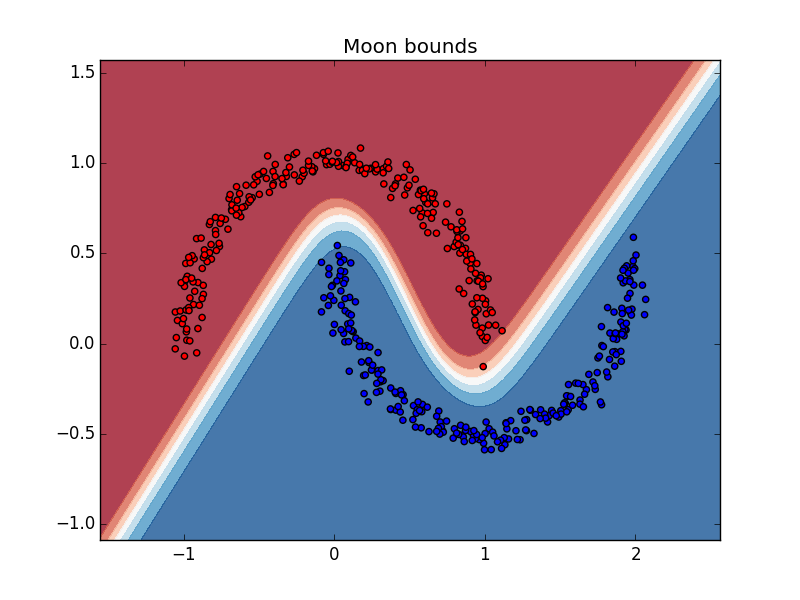
\includegraphics[width=\columnwidth]{fig/moon-bound-0.png}
\caption{Moon classique}
\end{figure}

On peut simuler un problème d'adaptation en appliquant une petite
transformation sur ces données.
Après une rotation de 35 degrés des données le réseau de base perd une bonne
partie de ses performances. On définit donc le domaine Source et Cible
comme étant respectivement les données originelles et les données après
rotation.

L'utilisation d'un \emph{DANN} permet de réduire en partie la perte de 
performance en adaptant le réseau à ces nouvelles données.

\begin{figure*}[htbp]
\centering
\subfigure[Sans le DANN les performances sont diminuées.]
	{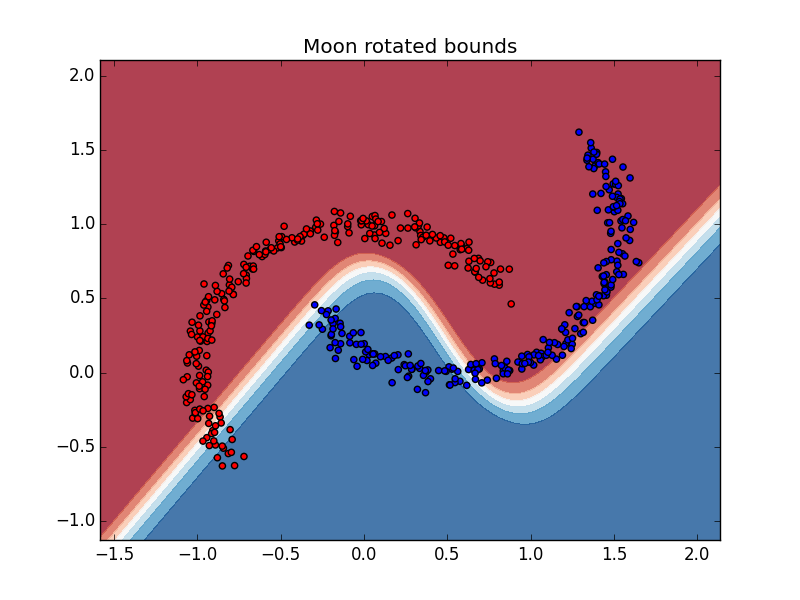
\includegraphics[width=\columnwidth]{fig/moon-rot-bound-0.png}}
\hfill
\subfigure[En applicant un DANN on peut partiellement corriger ce problème
($\lambda_D=0.7$)]
	{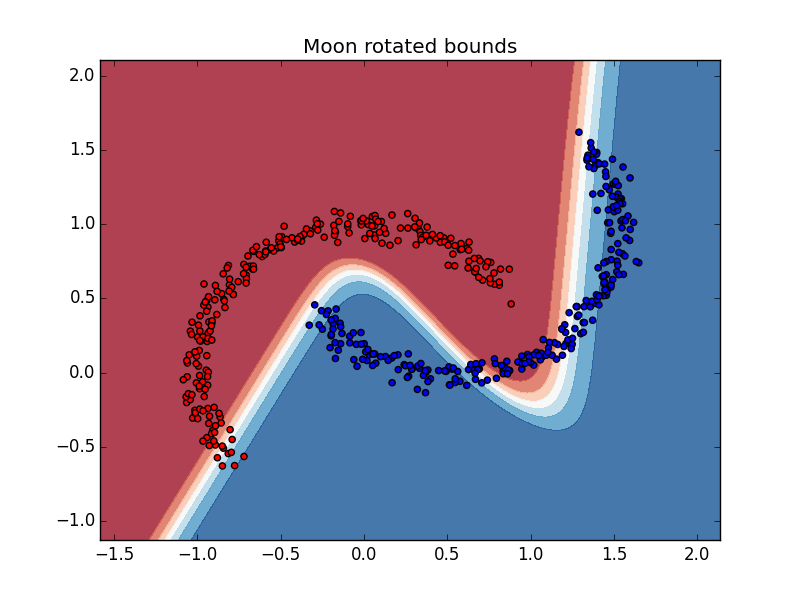
\includegraphics[width=\columnwidth]{fig/moon-rot-bound-1.png}}
\caption{Moon après une rotation de 35 degrés.}

\centering
\subfigure[Avant l'utilisation du DANN.]
	{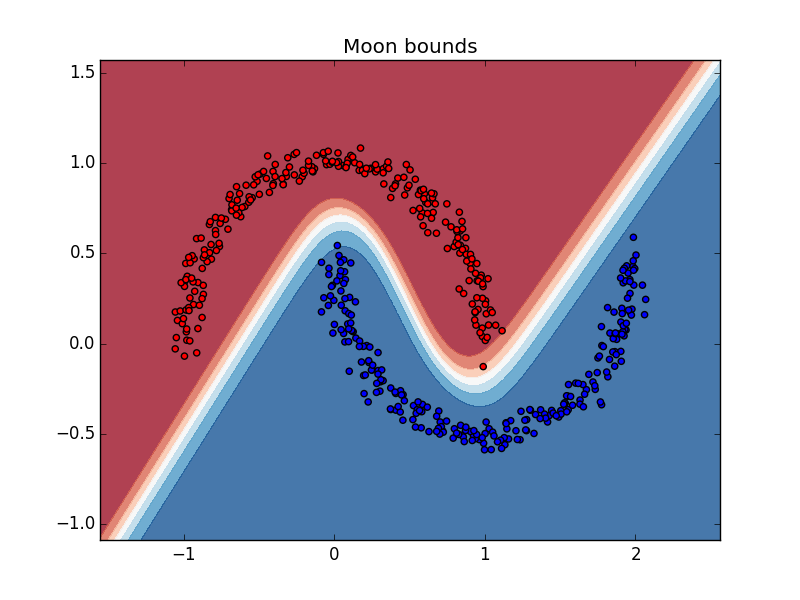
\includegraphics[width=\columnwidth]{fig/moon-bound-0.png}}
\hfill
\subfigure[Le DANN ne fait pas perdre de performances sur ces données.]
	{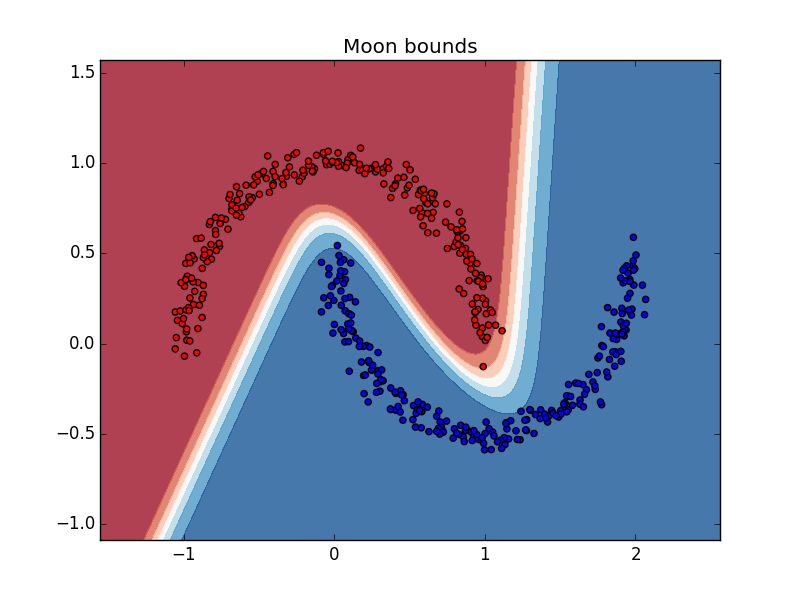
\includegraphics[width=\columnwidth]{fig/moon-bound-1.png}}
\caption{Moon (donnée originale).}
\end{figure*}

Une autre transformation consiste à appliquer une matrice à dominance
diagonale aux données:

\[ x \gets A.x \] où $A$ est une matrice $(2\times2)$ générée
aléatoirement.

\begin{figure*}[htbp]
\centering
\subfigure[Sans le DANN.]
	{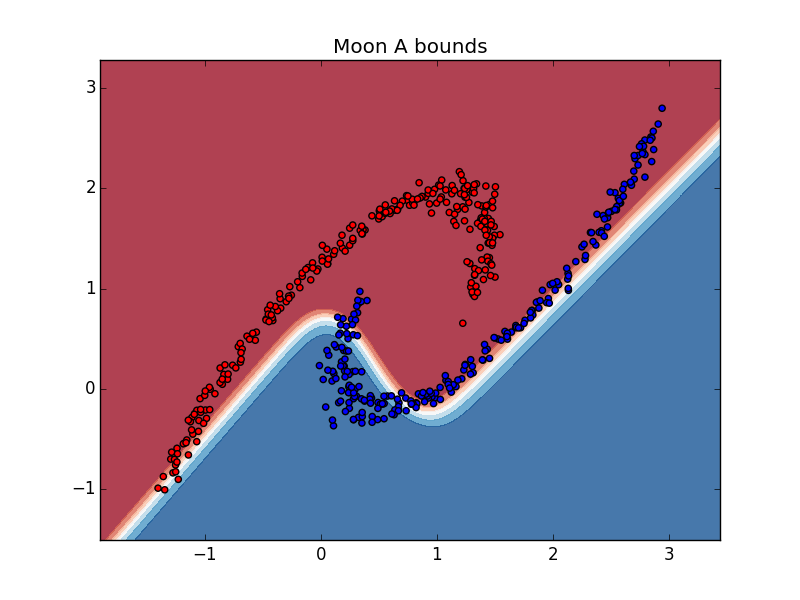
\includegraphics[width=\columnwidth]{fig/moon-A-bound-0.png}}
\hfill
\subfigure[En applicant un DANN ($\lambda_D=0.7$)]
	{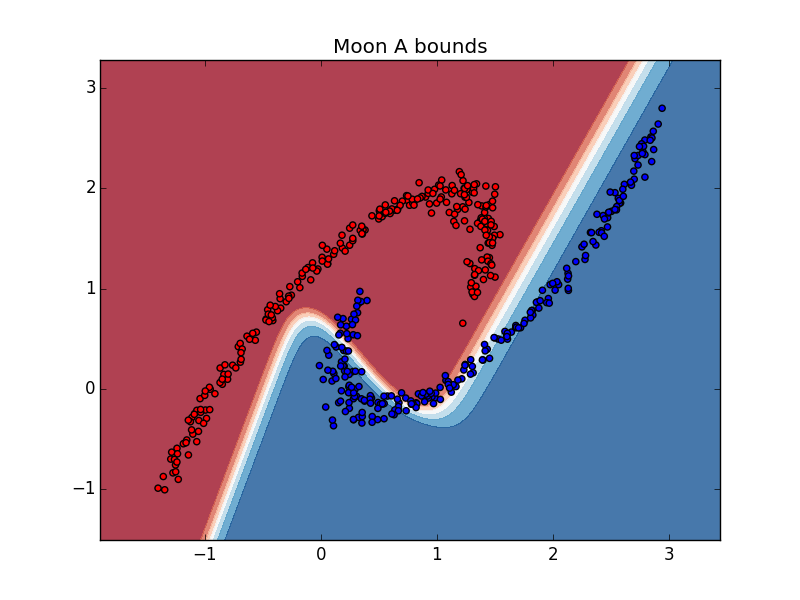
\includegraphics[width=\columnwidth]{fig/moon-A-bound-1.png}}
\caption{Moon après application de $A$.}
\end{figure*}


\FloatBarrier
% subsection moons (end)

\TODO Présenter les résultats sur MNIST "bruité" !
\TODO Pour faire ça il faudrait les matrices de confusion !

\TODO L'exemple de MNIST Miroir qui ne marche pas du tout avec un DANN sans
convolution mais qui ne nécessite pas d'aide avec une couche de convolution
\TODO Pour faire ça il faudrait les matrices de confusion !


